\documentclass[tikz,border=2pt]{standalone}
\usepackage{tikz}
\usetikzlibrary{positioning}
\begin{document}
% Namikawa--Ueno type: II_{(l+1)-0}
% Target MRNC type: I^*_{0,l}
% Adapted from Tim Dokchitser picture: I^*_{0,{\it n}}
% Parameter substitution: n -> l
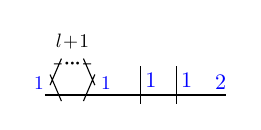
\begin{tikzpicture}[xscale=0.57,yscale=0.62]
\draw[thick,shorten >=2] (-0.09,0)--(4.07,0) node[inner sep=2pt,blue,above left,scale=0.8] {2};
\draw[scale=0.8] (0,0) ++(0.05,0.3) node[anchor=east,blue,scale=0.7] {1} ++(0.3,-0.45)--++(115:0.75)++(295:0.15)++(245:0.15)--++(65:0.75)++(245:0.15)++(180:0.15)--++(0:0.22) ++(0:0.15) node{$\cdot$} ++(0:0.15) node{$\cdot$} node[above=0.1,anchor=south,scale=0.7]{$l\!+\!1$}++(0:0.15) node{$\cdot$} ++(0:0.15) --++(0:0.22)++(180:0.15)++(115:0.15)--++(295:0.75)++(115:0.15)++(65:0.15)--++(245:0.75)++(0.3,0.45) node[anchor=west,blue,scale=0.7] {1};\draw[shorten <=-3pt] (2.04,0)--node[inner sep=2pt,scale=0.8,blue,right] {1} (2.04,3/5);
\draw[shorten <=-3pt] (2.84,0)--node[inner sep=2pt,scale=0.8,blue,right] {1} (2.84,3/5);
\end{tikzpicture}
\end{document}
